% !TEX root = task-3-4-8.tex
% Editable task bank. Append new BankTask blocks at the end of the document.
\documentclass[12pt,a4paper]{article}
\usepackage{physics-textbook}
\usepackage{graphicx,needspace}
\usetikzlibrary{decorations.pathmorphing}
\newif\ifShowSolutions
\ifdefined\TutorEdition
  \ShowSolutionstrue
\else
  \ShowSolutionsfalse % Change to \ShowSolutionstrue to display solutions.
\fi
\newcounter{banktask}
\newsavebox{\BankTaskBox}
\newcommand{\BankTaskContent}[3]{%
  \noindent\textbf{\thebanktask.}\quad #2\par
  \ifShowSolutions
    \Needspace{50mm}% Keep the solution heading with its opening text or diagram.
    #3\par
    \ifdefined\TutorEdition
      \ifcsname TutorSource#1\endcsname
        \nopagebreak\smallskip{\small\csname TutorSource#1\endcsname\par}%
      \fi
    \fi
  \fi
}
\newcommand{\BankTask}[3]{%
  \refstepcounter{banktask}\par\medskip
  \sbox{\BankTaskBox}{\begin{minipage}{\linewidth}%
    \BankTaskContent{#1}{#2}{#3}\end{minipage}}%
  \ifdim\dimexpr\ht\BankTaskBox+\dp\BankTaskBox\relax>\dimexpr\textheight-20mm\relax
    \Needspace{35mm}\BankTaskContent{#1}{#2}{#3}%
  \else
    \Needspace{\dimexpr\ht\BankTaskBox+\dp\BankTaskBox\relax}%
    \noindent\usebox{\BankTaskBox}\par
  \fi
  \medskip
}
\begin{document}
\BookSubsection{3.4.8}{Однородное поле: связь напряжения и напряжённости}


% Source sdamgia-1306: https://phys-ege.sdamgia.ru/problem?id=1306
\BankTask{sdamgia-1306}{
Какова разность потенциалов между точками поля, если при перемещении заряда $12 \,\text{мкКл}$ из одной точки в другую электростатическое поле совершает работу $0{,}36 \,\text{мДж}$? (В вольтах.)\par
}{
\smallskip\noindent\textbf{Решение}\par
Разность потенциалов представляет собой работу по переносу единичного заряда между точками поля. Следовательно, разность потенциалов равна $\frac{ 0{,}36\,\text{мДж}}{ 12\,\text{мкКл} } =30\,\text{В}.$\par
Ответ: $30$.\par
}

% Source sdamgia-1429: https://phys-ege.sdamgia.ru/problem?id=1429
\BankTask{sdamgia-1429}{
Модуль напряженности однородного электрического поля равен $100 \,\text{В/м}$. Каков модуль разности потенциалов между двумя точками, расположенными на одной силовой линии поля на расстоянии $5 \,\text{см}$? (В вольтах.)\par
}{
\smallskip\noindent\textbf{Решение}\par
Модуль разности потенциалов между точками, расположенными на одной силовой линии, связана с расстоянием между этими точками и напряженностью однородного электрического поля соотношением\par
\[U=E\Delta x=100\,\text{В/м} \cdot 0{,}05\,\text{м}=5\,\text{В}.\]
Ответ: $5$.\par
}

% Source sdamgia-4104: https://phys-ege.sdamgia.ru/problem?id=4104
\BankTask{sdamgia-4104}{
Двум металлическим пластинам площадью $S$ каждая сообщили равные по модулю, но противоположные по знаку заряды +$Q$ и -$Q$. Пластины расположили на малом расстоянии $d$ друг от друга. Установите соответствие между физическими величинами и формулами, по которым их можно рассчитать.\par

\begin{center}\begin{minipage}[t]{.47\linewidth}\textbf{Формулы}\par\smallskip $A$) $\frac{ Qd}{ \varepsilon_{0} S }$\par
Б) $\frac{ Q ^2 d}{ 2\varepsilon_{0} S }$\end{minipage}\hfill\begin{minipage}[t]{.47\linewidth}\textbf{Физические величины}\par\smallskip $1$. Напряженность электрического поля между пластинами\par
$2$. Разность потенциалов между пластинами\par
$3$. Емкость системы, состоящей из двух таких пластин\par
$4$. Энергия электрического поля, заключенного между этими пластинами\end{minipage}\end{center}
\par
\begin{center}\small\setlength{\tabcolsep}{3pt}\begin{tabular}{|p{0.45\linewidth}|p{0.45\linewidth}|}\hline
$A$ & Б\\\hline
 & \\\hline
\end{tabular}\end{center}\par
}{
\smallskip\noindent\textbf{Решение}\par
Описанная в задаче система представляет собой заряженный плоский конденсатор. Емкость такого конденсатора равна $C= \frac{ \varepsilon_{0} S}{ d } .$ Энергия плоского конденсатора дается выражением: $W= \frac{ Q ^2 }{ 2C } = \frac{ Q ^2 d}{ 2\varepsilon_{0} S } ,$ следовательно, формула Б описывает энергию электрического поля, заключенного между пластинами. Разность потенциалов между пластинами равна $U= \frac{ Q}{ C } = \frac{ Qd}{ \varepsilon_{0} S } .$ Следовательно, формуле А соответствует пункт $2$. Наконец, чтобы завершить разговор по поводу данной задачи, напомним выражение для напряженности электрического поля между пластинами: $E= \frac{ U}{ d } = \frac{ Q}{ \varepsilon_{0} S } .$\par
Ответ: $24$.\par
}

% Source sdamgia-10474: https://phys-ege.sdamgia.ru/problem?id=10474
\BankTask{sdamgia-10474}{
Две параллельные металлические пластины больших размеров расположены на расстоянии $d$ друг от друга и подключены к источнику постоянного напряжения (рис. $1$). Пластины закрепили на изолирующих подставках и спустя длительное время отключили от источника (рис. $2$).\par
$1$. Напряженность электрического поля в точке А больше, чем в точке В.\par
$2$. Потенциал электрического поля в точке А больше, чем в точке С.\par
$3$. Если увеличить расстояние между пластинами $d$, то напряженность электрического поля в точке С не изменится.\par
$4$. Если уменьшить расстояние между пластинами $d$, то заряд правой пластины не изменится.\par
$5$. Если пластины полностью погрузить в керосин, то энергия электрического поля конденсатора останется неизменной.\par

\begin{center}\begin{tikzpicture}[book diagram,>=stealth]
\foreach\shift in{0,4}{\begin{scope}[xshift=\shift cm]\draw[thick](0,0)--(0,2.6)(2,0)--(2,2.6);\draw[<->](0,3)--(2,3)node[midway,above]{$d$};\draw(0,2.6)--(0,3.2)(2,2.6)--(2,3.2);\end{scope}}\draw(0,1.3)--(-.8,1.3)--(-.8,-.8)--(.65,-.8);\draw(.65,-.8)circle(.1);\draw(1.35,-.8)circle(.1);\draw(1.35,-.8)--(2.8,-.8)--(2.8,1.3)--(2,1.3);\node[above]at(.65,-.7){$-$};\node[above]at(1.35,-.7){$+$};\node at(1,-1.3){Рис.\ 1};\draw(4,1.3)--(3.5,1.3)(6,1.3)--(6.5,1.3);\foreach\x/\y/\s in{4.55/.55/A,4.55/1.7/B,5.3/1.15/C}{\fill(\x,\y)circle(1.5pt);\node[above]at(\x,\y){$\s$};}\node at(5,-1.3){Рис.\ 2};
\end{tikzpicture}\end{center}
\par
}{
\smallskip\noindent\textbf{Решение}\par
После того как длительное время пластины были подключены к источнику постоянного напряжения, они зарядились: левая пластина — отрицательно, правая — положительно.\par
$1$. Внутри плоского заряженного конденсатора электрическое поле однородно. Напряженности поля в точках А и В одинаковые. Утверждение $1$ неверно.\par
$2$. Потенциал электрического поля внутри конденсатора убывает от положительной пластины к отрицательной. Потенциал электрического поля в точке А меньше, чем в точке С. Утверждение $2$ неверно.\par
$3$. Поскольку пластины отключены от источника, то заряд и его поверхностная плотность на них не меняется при изменении расстояния. Значит, не будет изменяться и напряженность электрического поля между пластинами. Утверждение $3$ верно.\par
$4$. Заряд пластин остается постоянным, независимо от того, сдвигают пластины или нет. Утверждение $4$ верно.\par
$5$. Диэлектрическая проницаемость керосина больше $1$. При полном погружении в керосин энергия электрического поля конденсатора $W= \frac{ q ^2 }{ 2C }$ уменьшится. Утверждение $5$ неверно.\par
Ответ: $34$.\par
}

% Source sdamgia-8876: https://phys-ege.sdamgia.ru/problem?id=8876
\BankTask{sdamgia-8876}{
Частица массой $0{,}08 \,\text{мг}$, имеющая заряд $10^{-10}\,\text{Кл}$, покоится в точке А. При включении горизонтального однородного электрического поля эта частица, двигаясь по горизонтали вдоль силовой линии, смещается в точку В. Напряжение между точками $A$ и $B$ равно $1 \,\text{В}$. Чему равна скорость частицы в точке В? (В метрах в секунду.)\par
}{
\smallskip\noindent\textbf{Решение}\par
Электрическое поле совершает работу по перемещению заряда: $A=qU.$\par
Работа по перемещению заряда равна изменению кинетической энергии $\Delta W_{\text{к}}= \frac{ m v ^2 }{ 2 } - \frac{ m v _{0} ^2 }{ 2 } ,$ причем, покоящаяся вначале частица кинетической энергией не обладала. Таким образом, получаем:\par
\[qU= \frac{ m v ^2 }{ 2 } .\]
Отсюда скорость частицы равна:\par
\[v=\sqrt{\frac{2qU}m}=\sqrt{\frac{2\cdot10^{-10}\cdot1}{0{,}08\cdot10^{-6}}}=0{,}05\,\text{м/с}.\]
Ответ: $0{,}05 \,\text{м/с}$.\par
}

% Source sdamgia-2990: https://phys-ege.sdamgia.ru/problem?id=2990
\BankTask{sdamgia-2990}{
Пылинка, имеющая массу $10 ^{ - 8 } \,\text{г}$ и заряд $( - 1{,}8 ) \cdot 10 ^{ - 14 } \,\text{Кл},$ влетает в электрическое поле вертикального плоского конденсатора в точке, находящейся посередине между его пластинами (см. рис., вид сверху).\par
Чему должна быть равна минимальная скорость, с которой пылинка влетает в конденсатор, чтобы она смогла пролететь его насквозь? Длина пластин конденсатора $10 \,\text{см}$, расстояние между пластинами $1 \,\text{см}$, напряжение на пластинах конденсатора $5000 \,\text{В}$. Система находится в вакууме. Действием силы тяжести пренебречь.\par

\begin{center}\begin{tikzpicture}[book diagram,>=stealth]
\draw(0,1.1)rectangle(5,1.4);\draw(0,-1.1)rectangle(5,-1.4);\foreach\x in{.4,1.4,...,4.4}{\node at(\x,1.25){$+$};\node at(\x,-1.25){$-$};}\draw[thin](.2,0)--(5,0);\draw[fill=white](.15,0)circle(.12);\draw[->,thick](.27,0)--(1.2,0)node[midway,above]{$\vec v$};
\end{tikzpicture}\end{center}
\par
}{
\smallskip\noindent\textbf{Решение}\par
Сила, действующая на частицу в конденсаторе со стороны поля: $F_{\text{эл}}=E|q|.$ Связь напряженности электрического поля с напряжением на пластинах конденсатора: $E= \frac{ U}{ d } ,$ где $d$ — расстояние между пластинами. Второй закон Ньютона в проекции на ось, перпендикулярную пластинам: $F_{\text{эл}}=ma,$ или $\frac{ |q|U}{ d } =ma.$\par
Рассмотрим движение частицы в электрическом поле конденсатора, выбрав оси: Ox вдоль пластины, Oy перпендикулярно вверх на рисунке. Так как пылинка отрицательная, то вектор электрической силы противоположно направлен с вектором напряженности (вверх), по второму закону Ньютона вектор ускорения сонаправлен с вектором силы. Таким образом, движение в поле конденсатора по оси Ox равномерное со скоростью $\upsilon$, перемещение $s_{x}$ равно длине пластин $l$. По оси Oy движение равноускоренное, причем проекция начальной скорости на ось Oy равна $0$, перемещение — $s_{y}.$\par
Сила со стороны электрического поля действует в вертикальном направлении, в вертикальной плоскости будет движение под действием этой силы, по параболе. Время полета вдоль пластин составляет $t= \frac{ l}{ v } .$ За это время частица сместится в сторону пластины на $s_{y}= \frac{ at ^2 }{ 2 } = \frac{ |q|Ul ^2 }{ 2dm v ^2 } .$ Условием пролета насквозь является $s \le \frac{ d}{ 2 } .$ Откуда получаем минимальную скорость:\par
\[v=\frac ld\sqrt{\frac{|q|U}{m}}=\frac{0{,}1}{0{,}01}\sqrt{\frac{1{,}8\cdot10^{-14}\cdot5000}{10^{-11}}}=30\,\text{м/с}.\]
Ответ: $v =30\,\text{м/с}.$\par
}

% Source sdamgia-2993: https://phys-ege.sdamgia.ru/problem?id=2993
\BankTask{sdamgia-2993}{
Маленький шарик с зарядом $q=4 \cdot 10 ^{ - 8 } \,\text{Кл}$ и массой $3 \,\text{г}$, подвешенный на невесомой нити с коэффициентом упругости $100 \,\text{Н/м}$, находится между вертикальными пластинами плоского воздушного конденсатора. Расстояние между обкладками конденсатора $5 \,\text{см}$. Какова разность потенциалов между обкладками конденсатора, если удлинение нити $0{,}5 \,\text{мм}$?\par

\begin{center}\begin{tikzpicture}[book diagram,>=stealth]
\draw[thick](-1.8,-1)--(-1.8,2.3)(1.1,-1)--(1.1,2.3);\draw(-1.4,2.4)--(.8,2.4);\foreach\x in{-1.4,-1.1,...,.7}\draw(\x,2.4)--++(.2,.2);\draw(0,2.4)--(-1.3,.2);\draw[fill=white](-1.3,.2)circle(.2);
\end{tikzpicture}\end{center}
\par
}{
\smallskip\noindent\textbf{Решение}\par
Изобразим силы, действующие на шарик:\par

\begin{center}\begin{tikzpicture}[book diagram,>=stealth]
\draw[thick](-1.8,-1)--(-1.8,2.3)(1.1,-1)--(1.1,2.3);\draw(-1.4,2.4)--(.8,2.4);\foreach\x in{-1.4,-1.1,...,.7}\draw(\x,2.4)--++(.2,.2);\draw(0,2.4)--(-1.3,.2);\draw[fill=white](-1.3,.2)circle(.2) (0,0)circle(.2);\node[above left]at(-1.3,.2){$+q$};\draw[->](0,2.4)--(-2.3,2.4)node[below]{$x$};\draw[->](0,2.4)--(0,-1.25)node[below]{$y$};\draw[->,thick](-1.3,.2)--(-1.3,-.7)node[right]{$m\vec g$};\draw[->,thick](-1.3,.2)--(-2.3,.2)node[above]{$\vec F_{\text{э}}$};\draw[->,thick](-1.3,.2)--(-.65,1.3)node[left]{$\vec F_{\text{упр}}$};\draw(0,1.65)arc(-90:-120:.75);\node at(-.22,1.48){$\alpha$};
\end{tikzpicture}\end{center}
\par
Шарик находится в равновесии, если выполняется условие $\vec{F}_{\text{упр}} + m \vec{g} + \vec{F}_{\text{э}}=0.$ По закону Гука модуль силы упругости $F_{\text{упр}}=k\Delta l.$ Сила, с которой электрическое поле действует на заряженное тело, равна по модулю $F_{\text{э}}=Eq$ и сонаправлена с вектором напряженности, так как заряд тела положительный.\par
Проекция условия равновесия на координатные оси:\par
Ox: $F_{\text{упр}} \cdot \sin \alpha =F_{\text{э}},$\par
Oy: $F_{\text{упр}} \cdot \cos \alpha =mg.$\par
Объединяя уравнения, получаем:\par
\[k\Delta l \cdot \sin \alpha =qE,\]
\[k\Delta l \cdot \cos \alpha =mg.\]
Возведем оба равенства в квадрат и сложим их: $( k\Delta l ) ^2 = ( mg ) ^2 + ( qE ) ^2 ,$ откуда:\par
\[E= \frac{ \sqrt{( k\Delta l ) ^2 - ( mg ) ^2} }{ q } .\]
Напряженность электрического поля в конденсаторе: $E= \frac{ U}{ d } .$\par
Таким образом, напряжение между обкладками конденсатора:\par
\[\begin{aligned}U&=\frac{d\sqrt{(k\Delta l)^2-(mg)^2}}q\\&=\frac{5\cdot10^{-2}\sqrt{(100\cdot5\cdot10^{-4})^2-(3\cdot10^{-3}\cdot10)^2}}{4\cdot10^{-8}}=50\,\text{кВ}.\end{aligned}\]
Ответ: $U=50\,\text{кВ}.$\par
}

% Source sdamgia-4511: https://phys-ege.sdamgia.ru/problem?id=4511
\BankTask{sdamgia-4511}{
Ион ускоряется в электрическом поле с разностью потенциалов $U = 10\,\text{кВ}$ и попадает в однородное магнитное поле перпендикулярно к вектору его индукции $\vec{B}$ (см. рис.). Радиус траектории движения иона в магнитном поле $R = 0{,}2\,\text{м}$, модуль индукции магнитного поля равен $0{,}5 \,\text{Тл}$. Определите отношение массы иона к его электрическому заряду $\frac{ m}{ q } .$ Кинетической энергией иона при его вылете из источника пренебрегите.\par

\begin{center}\begin{tikzpicture}[book diagram,>=stealth]
\draw(-2,0)--(-2,1.1)--(-.8,1.1)--(-.8,.85);\draw(-2,0)--(-.8,0)--(-.8,.35);\draw(-.8,0)--(-.8,-.5)--(-.3,-.5);\draw(-.3,-.5)circle(.11);\draw(.3,-.5)circle(.11);\draw(.3,-.5)--(.7,-.5)--(.7,-.1);\draw(-.42,-.65)--(-.18,-.35)(.18,-.65)--(.42,-.35);\node[below]at(-.3,-.6){$+$};\node[below]at(.3,-.6){$-$};\draw[->,thick](-.8,.6)--(1.1,.6);\node[below]at(.15,.6){$U$};\draw[dashed](1.1,-.8)--(1.1,1.6);\foreach\x in{1.5,2.1,2.7}\foreach\y in{-.3,.4,1.1}{\draw(\x,\y)circle(.13);\fill(\x,\y)circle(1pt);}\node at(2,-.8){$\vec B$};\node[below left,align=left]at(-.8,-.15){Источник\\ионов};
\end{tikzpicture}\end{center}
\par
}{
\smallskip\noindent\textbf{Решение}\par
Разность потенциалов сообщает иону кинетическую энергию $W= \frac{ m v ^2 }{ 2 } .$ При этом изменение кинетической энергии равно работе электрического поля $A=qU.$ Откуда получаем:\par
\[v ^2 =2U \frac{ q}{ m } .\]
В магнитном поле, на движущийся ион действует сила Лоренца $F_{\text{л}}=Bq v \sin \alpha ,$ где $\sin \alpha =1,$ которая сообщает ему центростремительное ускорение $a= \frac{ v ^2 }{ R } .$ По второму закону Ньютона $F_{\text{л}}=ma.$\par
Объединяя формулы, находим:\par
\[v ^2 = ( \frac{ q}{ m } ) ^2 B ^2 R ^2 .\]
Приравнивая правые части полученных равенств, находим искомое отношение массы к заряду:\par
\[\frac{ m}{ q } = \frac{ B ^2 R ^2 }{ 2U } = \frac{ ( 0{,}5\,\text{Тл} ) ^2 ( 0{,}2\,\text{м} ) ^2 }{ 2 \cdot 10000\,\text{В} } =5 \cdot 10 ^{ - 7 } \,\text{кг/Кл}.\]
Ответ: $5 \cdot 10 ^{ - 7 } \,\text{кг/Кл}.$\par
}


% Source 410957: https://ege.fipi.ru/bank/questions.php?search=1&proj=BA1F39653304A5B041B656915DC36B38&qid=410957
\BankTask{410957}{
Две параллельные металлические пластины больших размеров расположены на расстоянии \(d\) друг от друга и подключены к источнику постоянного напряжения (рис. 1). Пластины закрепили на изолирующих подставках и спустя длительное время отключили от источника (рис. 2).
\begin{enumerate}
\item Напряжённость электрического поля в точке \(B\) больше, чем в точке \(C\).
\item Потенциалы электрического поля в точках \(A\) и \(B\) одинаковы.
\item Если после отключения от источника увеличить расстояние \(d\) между пластинами, то напряжённость электрического поля в точке \(A\) увеличится.
\item Если после отключения от источника уменьшить расстояние \(d\) между пластинами, то заряд правой пластины не изменится.
\item Если после отключения от источника пластины полностью погрузить в керосин, то энергия электрического поля системы пластин уменьшится.
\end{enumerate}
\begin{center}
\begin{tikzpicture}[book diagram,x=0.8cm,y=0.8cm]
\draw[very thick] (0,0.7)--(0,3.5) (1.25,0.7)--(1.25,3.5);
\draw[thin] (0,3.5)--(0,4.35) (1.25,3.5)--(1.25,4.35);
\draw[{book tip}-{book tip}] (0,3.9)--(1.25,3.9) node[midway,above] {$d$};
\draw (0,1.85)--(-1.1,1.85)--(-1.1,-0.2)--(0.35,-0.2);
\draw (1.25,1.85)--(2.35,1.85)--(2.35,-0.2)--(0.9,-0.2);
\draw[fill=white] (0.35,-0.2) circle (0.065) (0.9,-0.2) circle (0.065);
\node[above] at (0.35,-0.15) {$-$};
\node[above] at (0.9,-0.15) {$+$};
\node at (0.625,-0.8) {Рис. 1};
\begin{scope}[xshift=4.7cm]
\draw[very thick] (0,0.7)--(0,3.5) (1.25,0.7)--(1.25,3.5);
\draw[thin] (0,3.5)--(0,4.35) (1.25,3.5)--(1.25,4.35);
\draw[{book tip}-{book tip}] (0,3.9)--(1.25,3.9) node[midway,above] {$d$};
\draw (0,1.85)--(-0.9,1.85) (1.25,1.85)--(2.15,1.85);
\fill (0.35,2.35) circle (0.045) node[above left] {$B$};
\fill (0.98,1.85) circle (0.045) node[above left] {$C$};
\fill (0.65,1.15) circle (0.045) node[left] {$A$};

\node at (0.625,-0.8) {Рис. 2};
\end{scope}
\end{tikzpicture}
\end{center}
}{
\smallskip\noindent\textbf{Решение от GPT}\par
Между большими параллельными пластинами поле однородно, поэтому \(E_B=E_C\) и утверждение 1 неверно. Точки \(A\) и \(B\) находятся на разных расстояниях от пластин, поэтому их потенциалы различаются: утверждение 2 неверно. После отключения заряд сохраняется, а \(E=Q/(\varepsilon_0S)\) не зависит от \(d\), поэтому утверждение 3 неверно, а 4 верно. При погружении в керосин ёмкость увеличивается в \(\varepsilon\) раз, а энергия \(W=Q^2/(2C)\) уменьшается в \(\varepsilon\) раз, поэтому утверждение 5 верно. Ответ: \(4,\ 5\).
}

% Source 19854: https://phys-ege.sdamgia.ru/problem?id=19854
\BankTask{19854}{
\begin{center}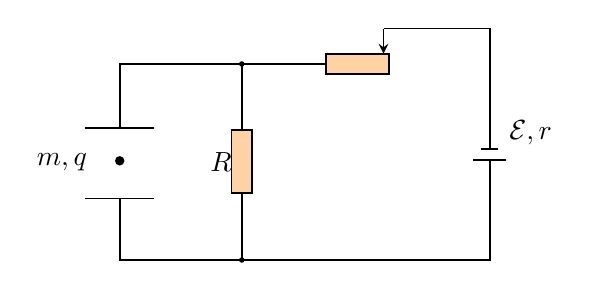
\begin{tikzpicture}[>=stealth,line width=.6pt]

\draw(0,1.17)--(0,1.98)--(2.62,1.98) (0,.27)--(0,-.51)--(4.7,-.51)--(4.7,.76)
 (4.7,.90)--(4.7,2.43)--(3.35,2.43);
\draw[->](3.35,2.43)--(3.35,2.11);
\draw(-.44,1.17)--(.44,1.17) (-.44,.27)--(.44,.27);
\draw(1.55,1.98)--(1.55,1.14) (1.55,.34)--(1.55,-.51);
\fill(0,.75)circle(.06) (1.55,1.98)circle(.035) (1.55,-.51)circle(.035);
\begin{scope}[shift={(3.02,1.98)},rotate=0]\draw[fill=orange!35] (-.4,-.13) rectangle (.4,.13);\end{scope}\begin{scope}[shift={(1.55,0.74)},rotate=90]\draw[fill=orange!35] (-.4,-.13) rectangle (.4,.13);\end{scope}\node[left] at (1.55,0.74) {$R$};\begin{scope}[shift={(4.7,0.83)},rotate=90]\draw(-.07,-.21)--(-.07,.21) (.07,-.11)--(.07,.11);\end{scope}\node[above right] at (4.82,0.83) {$\mathcal E,r$};\node[left]at(-.29,.73){$m,q$};
\end{tikzpicture}\end{center}
Две параллельные металлические пластины, расположенные горизонтально, подключены к электрической схеме, приведенной на рисунке. Между пластинами находится в равновесии маленькое заряженное тело массой m и зарядом q. Электростатическое поле между пластинами считать однородным. Опираясь на законы механики и электродинамики, объясните, как и в какую сторону начнет двигаться тело, если сдвинуть ползунок реостата влево.
}{
\smallskip\noindent\textbf{Решение}\par
\begin{center}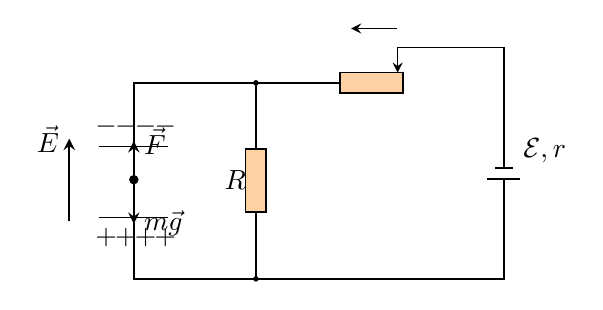
\begin{tikzpicture}[>=stealth,line width=.6pt]

\draw(0,1.17)--(0,1.98)--(2.62,1.98) (0,.27)--(0,-.51)--(4.7,-.51)--(4.7,.76)
 (4.7,.90)--(4.7,2.43)--(3.35,2.43);
\draw[->](3.35,2.43)--(3.35,2.11);
\draw(-.44,1.17)--(.44,1.17) (-.44,.27)--(.44,.27);
\draw(1.55,1.98)--(1.55,1.14) (1.55,.34)--(1.55,-.51);
\fill(0,.75)circle(.06) (1.55,1.98)circle(.035) (1.55,-.51)circle(.035);
\begin{scope}[shift={(3.02,1.98)},rotate=0]\draw[fill=orange!35] (-.4,-.13) rectangle (.4,.13);\end{scope}\begin{scope}[shift={(1.55,0.74)},rotate=90]\draw[fill=orange!35] (-.4,-.13) rectangle (.4,.13);\end{scope}\node[left] at (1.55,0.74) {$R$};\begin{scope}[shift={(4.7,0.83)},rotate=90]\draw(-.07,-.21)--(-.07,.21) (.07,-.11)--(.07,.11);\end{scope}\node[above right] at (4.82,0.83) {$\mathcal E,r$};
\foreach \x in {-.35,-.1,.15,.4}{\node at(\x,1.43){$-$};\node at(\x,.02){$+$};}
\draw[->,thick] (0,.75)--(0,.19)node[right]{$m\vec g$};
\draw[->,thick] (0,.75)--(0,1.24)node[right]{$\vec F$};
\draw[->,thick](-.82,.23)--(-.82,1.27)node[left]{$\vec E$};
\draw[->](3.34,2.67)--(2.76,2.67);

\end{tikzpicture}\end{center}
$1$.  Поскольку пластины подключены к источнику ЭДС, то между ними имеется разность потенциалов, в пространстве между ними создается однородное электростатическое поле. Согласно электрической схеме, нижняя пластина имеет положительный заряд, а верхняя  — отрицательный; следовательно, вектор напряженности поля направлен вертикально вверх. По условию задачи заряженное тело находится в равновесии; следовательно, сила тяжести скомпенсирована силой Кулона, направленной вертикально вверх. Отсюда делаем вывод, что тело имеет положительный заряд.
$2$.  Если сдвинуть ползунок реостата влево, то сопротивление реостата уменьшится. Поскольку реостат соединен с резистором R последовательно, то и общее сопротивление цепи также уменьшится. 
$3$.  Согласно закону Ома для полной цепи $\mathcal{E}=I ( R_{\,\text{цепи}} + r )$  — при уменьшении сопротивления внешней цепи сила тока в ней увеличится. Таким образом, по закону Ома для участка цепи цепи $U=IR$  — напряжение на резисторе R также увеличится. Поскольку пластины соединены с резистором R параллельно, то, соответственно, напряжение между ними увеличится. Следовательно, увеличится и напряженность поля между пластинами: $E=U/d.$
$4$.  Увеличение напряженности поля приведет к увеличению силы Кулона, действующей на тело: $F=qE.$ Равновесие нарушится, сила Кулона станет больше силы тяжести, и тело начнет двигаться вверх с ускорением.
}

% Source 25399: https://phys-ege.sdamgia.ru/problem?id=25399
\BankTask{25399}{
\begin{center}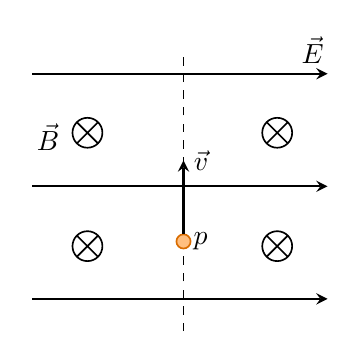
\begin{tikzpicture}[>=stealth,line width=.6pt]

\foreach \y in {-.9,.53,1.96}{\draw[->,thick](-1.68,\y)--(2.07,\y);}
\node[above]at(1.88,1.96){$\vec E$};
\foreach \x in {-.98,1.43}\foreach \y in {-.23,1.21}{\draw(\x,\y)circle(.19) (\x-.13,\y-.13)--(\x+.13,\y+.13) (\x-.13,\y+.13)--(\x+.13,\y-.13);}
\node[left]at(-1.21,1.15){$\vec B$};
\draw[dashed](.24,-1.31)--(.24,2.27);
\filldraw[fill=orange!50,draw=orange!85!black](.24,-.17)circle(.09) node[right]{$p$};
\draw[->,thick](.24,-.07)--(.24,.86)node[right]{$\vec v$};

\end{tikzpicture}\end{center}
В камере, из которой откачан воздух, создали электрическое поле напряженностью $\vec{E}$ и магнитное поле с индукцией $\vec{B}.$ Поля однородные, $\vec{E}\perp\vec{B}.$ В камеру влетает протон p, вектор скорости которого перпендикулярен $\overrightarrow{B}$ и $\overrightarrow{E}$ как показано на рисунке. Модули напряженности электрического поля и индукции магнитного поля таковы, что протон движется прямолинейно. Куда отклонится протон на начальном участке траектории, если его скорость уменьшить? Ответ поясните, указав, какие явления и закономерности Вы использовали для объяснения. Влиянием силы тяжести пренебречь.
}{
\smallskip\noindent\textbf{Решение}\par
На протон действует две силы: со стороны электрического поля $F_{\,\text{э}}=qE,$ направленная вправо, так как протон имеет положительный заряд; со стороны магнитного поля сила Лоренца $F_L=Bq v ,$ направленная влево по правилу левой руки. Протон движется равномерно, так как силы равны по модулю и противоположны, то есть равнодействующая этих сил равна $0$.
Если уменьшить скорость протона, то сила электрического поля не изменится, а сила Лоренца уменьшится. Тогда равнодействующая сила будет направлена вправо. Поскольку сила перпендикулярна скорости, то протон будет двигаться по криволинейной траектории, похожей на дугу окружности на начальном участке, отклоняясь вправо.
}

% Source 29880: https://phys-ege.sdamgia.ru/problem?id=29880
\BankTask{29880}{
\begin{center}\begin{tikzpicture}[>=stealth,line width=.55pt]\draw(0,-.48)arc(-140:-68:1.35) (-.3,-.13)arc(-140:-68:1);\draw[orange!85!black,->](1.41,-1.06)arc(-65:-159:1.15);\draw[->,orange!85!black](2.9,-1.07)--(1.6,-1.07);\draw(2.93,-1.34)rectangle(3.97,-.83)node[pos=.5]{И. Ч.};\draw(.1,-.58)--(.1,-1.87)--(5.03,-1.87)--(5.03,-.96) (-.18,-.31)--(5.03,-.31)--(5.03,-.63);\draw(5.03,-.7)circle(.07) (5.03,-.88)circle(.07);\node[right]at(5.12,-.8){$U$};\end{tikzpicture}\end{center}На рисунке показана схема устройства для предварительного отбора заряженных частиц для последующего детального исследования. Устройство представляет собой конденсатор, пластины которого изогнуты дугой радиусом $R.$ Перед попаданием в это пространство молекулы теряют один электрон. Во сколько раз надо изменить напряжение на обкладках конденсатора, чтобы сквозь него пролетали ионы, потерявшие два электрона? Влиянием силы тяжести пренебречь.
}{
\smallskip\noindent\textbf{Решение}\par
Центростремительное ускорение иона в конденсаторе $a= \frac{v ^2}{R}$ задается силой $F=qE= \frac{qU}{d}$ действия электрического поля, так что $\frac{qU}{d} =m \frac{v ^2}{R}$ (здесь q, m и \ensuremath{\upsilon} — соответственно заряд, масса и скорость иона; U  — напряжение на обкладках конденсатора, d  — расстояние между пластинами).
Тогда данное выражение имеет вид для каждого случая: 

$\frac{m v ^2}{R} = \frac{qU_1}{d}$ и $\frac{m v ^2}{R} = \frac{2qU_2}{d}$

Из соотношения видно, что для отбора ионов, потерявших два электрона, напряжение нужно уменьшить в $2$ раза.

Ответ:уменьшить в $2$ раза.
}

\end{document}
